\documentclass{article}
\usepackage{graphicx} % Required for inserting images
\usepackage[polish]{babel}
\usepackage[T1]{fontenc}
\usepackage{lipsum} % Pakiet do generowania tekstu 'Lorem ipsum'
\usepackage{geometry}

\title{JIMP2 Sprawozdanie z projektu w języku Java}
\author{Stanisław Dutkiewicz, Filip Kobus}
\date{Maj 2024}

\geometry{
  top=3.7cm, % Górny margines
  bottom=3.7cm, % Dolny margines
  left=4.7cm, % Lewy margines
  right=4.7cm, % Prawy margines
}

\begin{document}
\maketitle

\newpage
\tableofcontents

\newpage

\section{Wstęp}
Celem projektu jest opracowanie programu, który pozwala na znalezienie drogi we wczytanym labiryncie, na przykład najkrótszej ścieżki od wejścia do wyjścia. Labirynt jest udostępniany w postaci pliku tekstowego lub binarnego, a stworzony w Javie program, odpowiada za wczytanie labiryntu, znalezienie ścieżki oraz zapisanie labiryntu i ścieżki do pliku.

\subsection{Problem Zadania}

Głównym wyzwaniem projektu jest opracowanie przejrzystego interfejsu graficznego, który pozwoli użytkownikowi na bezproblemowe poruszanie się po funkcjonalnościach aplikacji oraz stworzenie efektywnej animacji przedstawiającej działanie algorytmów.

Dodatkowym wymaganiem jest efektywne zarządzanie zasobami systemowymi podczas przetwarzania dużych labiryntów, mimo że w przypadku aplikacji w języku Java nie ma bezpośredniego limitu zużycia pamięci. Ważne jest jednak, aby program działał sprawnie i szybko, nawet dla labiryntów o maksymalnym rozmiarze 1024x1024. Wyzwanie to wymaga implementacji skutecznych algorytmów przeszukiwania oraz optymalnego projektowania struktur danych używanych w programie.

\subsection{Sposób rozwiązania}

Do rozwiązania tego problemu wykorzystane zostaną dwie metody przeszukiwania: BFS (Breadth-First Search) oraz DFS (Depth-First Search), z których użytkownik może wybrać jeden. Algorytmy te posłużą do eksploracji labiryntu w celu znalezienia rozwiązania.


\vspace{1mm}

\item \textbf{DFS} jest to algorytm, który eksploruje labirynt, poruszając się zgodnie z ustalonymi wcześniej priorytetami ruchów (omijając przy tym ściany), a gdy napotka ślepy zaułek, cofa się do ostatnio napotkanego węzła, aby spróbować innej ścieżki. Algorytm został zaimplementowany w postaci iteracyjnej, mającej przewagę nad postacią rekurencyjną przez znacznie niższe zużycie zasobów.

\item \textbf{BFS} algorytm polega na przeszukiwaniu labiryntu wszerz, zapisując na stworzonej wcześniej kolejce możliwe do przejścia komórki, a następnie sukcesywnie odwiedzając każdą z nich co tym samym pozwoli na znalezienie najkrótsze drogi do wyjścia. Jego przewagą na algorytmem DFS jest pewność znalezienia najkrótszej ścieżki, co w DFS zależy od ustawień początkowych oraz konfiguracji ścian labiryntu.

\vspace{5mm}

Implementacja tych algorytmów w języku Java, którą opracowaliśmy, wymagała szczególnej uwagi na efektywne zarządzanie pamięcią. Aby sprostać temu wyzwaniu, kluczowe okazało się nie tylko zaprojektowanie samych algorytmów, ale również efektywne przechowywanie struktur danych, takich jak stosy i kolejki, które służą do zapamiętywania odwiedzonych komórek i ścieżek w labiryncie.

\subsection{Rodzaje plików wejściowych}

\item \textbf{Plik tekstowy}: Zawiera symbole reprezentujące elementy labiryntu tj. wejście do labiryntu (P), wyjście z labiryntu (K), ściany (X) oraz miejsca, po których można się poruszać (spacja).

\item \textbf{Plik binarny}: Składa się z nagłówka pliku, informującego o: rozmiarach labiryntu, współrzędnych wejścia i wyjścia oraz binarnych reprezentacjach elementów labiryntu (takich samych jak te w wersji tekstowej). Następnie zamiesczono w niej sam labirynt w postaci przypominającej wersję tekstową z niewielką różnicą tzn. przed informacją o rodzaju komórki (ściana lub wolna przestrzeń), umieszczona została liczba jego wystąpień w danym miejscu co pozwoliło na znaczne ograniczenie rozmiarów pliku wejściowego. Ostatnim elementem pliku jest sekcja rozwiązania gdzie autor labiryntu może zamieścić rozwiązanie do labiryntu, choć nie jest to wymagane.

\section{Implementacja}

Implementacja projektu, realizowanego w języku Java, skupiła się na rozwiązaniu problemu nawigacji przez labirynt z użyciem algorytmu przeszukiwania w głąb (DFS) oraz w szerz (BFS), przy jednoczesnym ograniczeniu zużycia pamięci. Kluczową decyzją projektową była modularna architektura systemu, która ułatwiła zarządzanie kodem oraz optymalizację pamięci. Poniżej są przedstawione kluczowe moduły projektu, które razem tworzą spójny system zdolny do skutecznego rozwiązywania labiryntów.

\subsection{Moduły}

\textbf{Moduł \texttt{AlgorithmBfs}}: Moduł \texttt{AlgorithmBfs} implementuje algorytm przeszukiwania wszerz (BFS) do znajdowania ścieżki w labiryncie.

\begin{itemize}
  \item \texttt{queue}: kolejka przechowująca punkty do odwiedzenia.
  \item \texttt{runAlgorithm()}: metoda uruchamiająca algorytm BFS.
  \item \texttt{addPossibleMovesToQueue(Point point)}: metoda dodająca możliwe ruchy do kolejki.
\end{itemize}

\textbf{Moduł \texttt{AlgorithmDfs}}: Moduł \texttt{AlgorithmDfs} implementuje algorytm przeszukiwania w głąb (DFS) do znajdowania ścieżki w labiryncie.

\begin{itemize}
  \item \texttt{stack}: stos przechowujący punkty do odwiedzenia.
  \item \texttt{makeMove()}: metoda wykonująca jeden krok algorytmu DFS.
  \item \texttt{getMove()}: metoda zwracająca ostatni wykonany ruch.
\end{itemize}

\textbf{Moduł \texttt{Binary}}: Moduł \texttt{Binary} odpowiada za konwersję labiryntu z formatu binarnego do formatu tekstowego.

\begin{itemize}
  \item \texttt{readUnsignedShortLittleEndian(DataInputStream dis)}: metoda odczytująca 2 bajty z pliku binarnego w kolejności little-endian.
  \item \texttt{convertBinaryToText(String binaryFilePath, String textFilePath)}: metoda konwertująca plik binarny do formatu tekstowego.
  \item \texttt{generateMazeFromEncoding(DataInputStream binaryFile, BufferedWriter textFile, long wordCount, int separator, int wall, int path, int cols, int rows, int entryX, int entryY, int exitX, int exitY)}: metoda generująca labirynt na podstawie kodowania binarnego.
\end{itemize}

\textbf{Moduł \texttt{DataArray}}: Moduł \texttt{DataArray} reprezentuje strukturę danych przechowującą labirynt.

\begin{itemize}
  \item \texttt{array}: tablica dwuwymiarowa przechowująca stan każdej komórki labiryntu.
  \item \texttt{putPointIntoArray(Point point)}: metoda umieszczająca punkt w tablicy.
  \item \texttt{setAsVisited(Point point)}: metoda oznaczająca punkt jako odwiedzony.
\end{itemize}

\textbf{Moduł \texttt{Point}}: Moduł \texttt{Point} reprezentuje punkt w labiryncie, przechowując jego współrzędne, typ i rodzica.

\begin{itemize}
  \item \texttt{x}: współrzędna x punktu.
  \item \texttt{getX()}: metoda zwracająca współrzędną x punktu.
  \item \texttt{movePoint(int xDiff, int yDiff)}: metoda przesuwająca punkt o podane różnice.
\end{itemize}

\textbf{Moduł \texttt{FileIO}}: Moduł \texttt{FileIO} zajmuje się wczytywaniem i zapisywaniem labiryntów w formacie tekstowym i binarnym.

\begin{itemize}
  \item \texttt{readMazeFromFile(File file)}: metoda wczytująca labirynt z pliku.
  \item \texttt{writeMazeToFile(BufferedImage image, File file)}: metoda zapisująca labirynt do pliku.
  \item \texttt{saveMazeAsText(BufferedImage mazeImage, JFrame window)}: metoda zapisująca labirynt jako plik tekstowy.
\end{itemize}

\textbf{Moduł \texttt{MainGuiPanel}}: Moduł \texttt{MainGuiPanel} jest odpowiedzialny za interfejs graficzny użytkownika oraz zarządzanie panelem głównym aplikacji.

\begin{itemize}
  \item \texttt{mazeRenderer}: obiekt klasy \texttt{MazeRenderer} do renderowania labiryntu.
  \item \texttt{run()}: metoda uruchamiająca główny panel GUI.
  \item \texttt{openMaze()}: metoda otwierająca plik z labiryntem.
\end{itemize}

\textbf{Moduł \texttt{MazeRenderer}}: Moduł \texttt{MazeRenderer} odpowiada za renderowanie labiryntu w interfejsie graficznym.

\begin{itemize}
  \item \texttt{mazeImage}: obraz labiryntu.
  \item \texttt{createMazePanel()}: metoda tworząca panel z labiryntem.
  \item \texttt{solveMazeWithBfs(DataArray dataArray)}: metoda rozwiązująca labirynt za pomocą algorytmu BFS.
\end{itemize}

\textbf{Moduł \texttt{MazeUtilities}}: Moduł \texttt{MazeUtilities} zawiera pomocnicze funkcje do obsługi labiryntu, takie jak sprawdzanie punktów wejścia i wyjścia.

\begin{itemize}
  \item \texttt{setSelectedState(state: int)}: metoda ustawiająca stan wyboru punktu.
  \item \texttt{handleMazeCellSelection(MazeRenderer mazeRenderer, int imageX, int imageY, JFrame window)}: metoda obsługująca wybór komórki labiryntu.
  \item \texttt{resetEntranceAndExit(MazeRenderer mazeRenderer, JFrame window)}: metoda resetująca punkty wejścia i wyjścia w labiryncie.
\end{itemize}

\textbf{Moduł \texttt{Main}}: Moduł \texttt{Main} jest główną klasą uruchamiającą aplikację.

\begin{itemize}
  \item \texttt{main(String[] args)}: metoda główna uruchamiająca aplikację.
\end{itemize}

\subsection{Wzorce projektowe}

\begin{itemize}
  \item \texttt{Singleton}: Moduł \texttt{FileIO}: Klasa \texttt{FileIO} ma prywatny konstruktor, co sugeruje użycie wzorca Singleton, aby zapewnić, że tylko jedna instancja tej klasy będzie używana w programie.
  
  \item \texttt{Singleton}: Algorytmy \texttt{AlgorithmBfs} i \texttt{AlgorithmDfs}: Klasy te implementują różne algorytmy przeszukiwania (BFS i DFS). Można je traktować jako różne strategie rozwiązania problemu nawigacji w labiryncie, które można łatwo zamieniać w zależności od potrzeb.
  
  \item \texttt{Composite}: Klasa \texttt{DataArray} przechowuje strukturę labiryntu jako tablicę punktów (\texttt{Point}). Wzorzec Composite jest stosowany w sposobie, w jaki poszczególne komórki labiryntu są traktowane jako elementy składowe większej struktury.
\end{itemize}


\subsection{Diagram Klas}
Poniżej przedstawiono diagram klas stworzony w programie Lucidchart:

\newgeometry{top=3.7cm, bottom=3.7cm, left=3cm, right=3cm}
    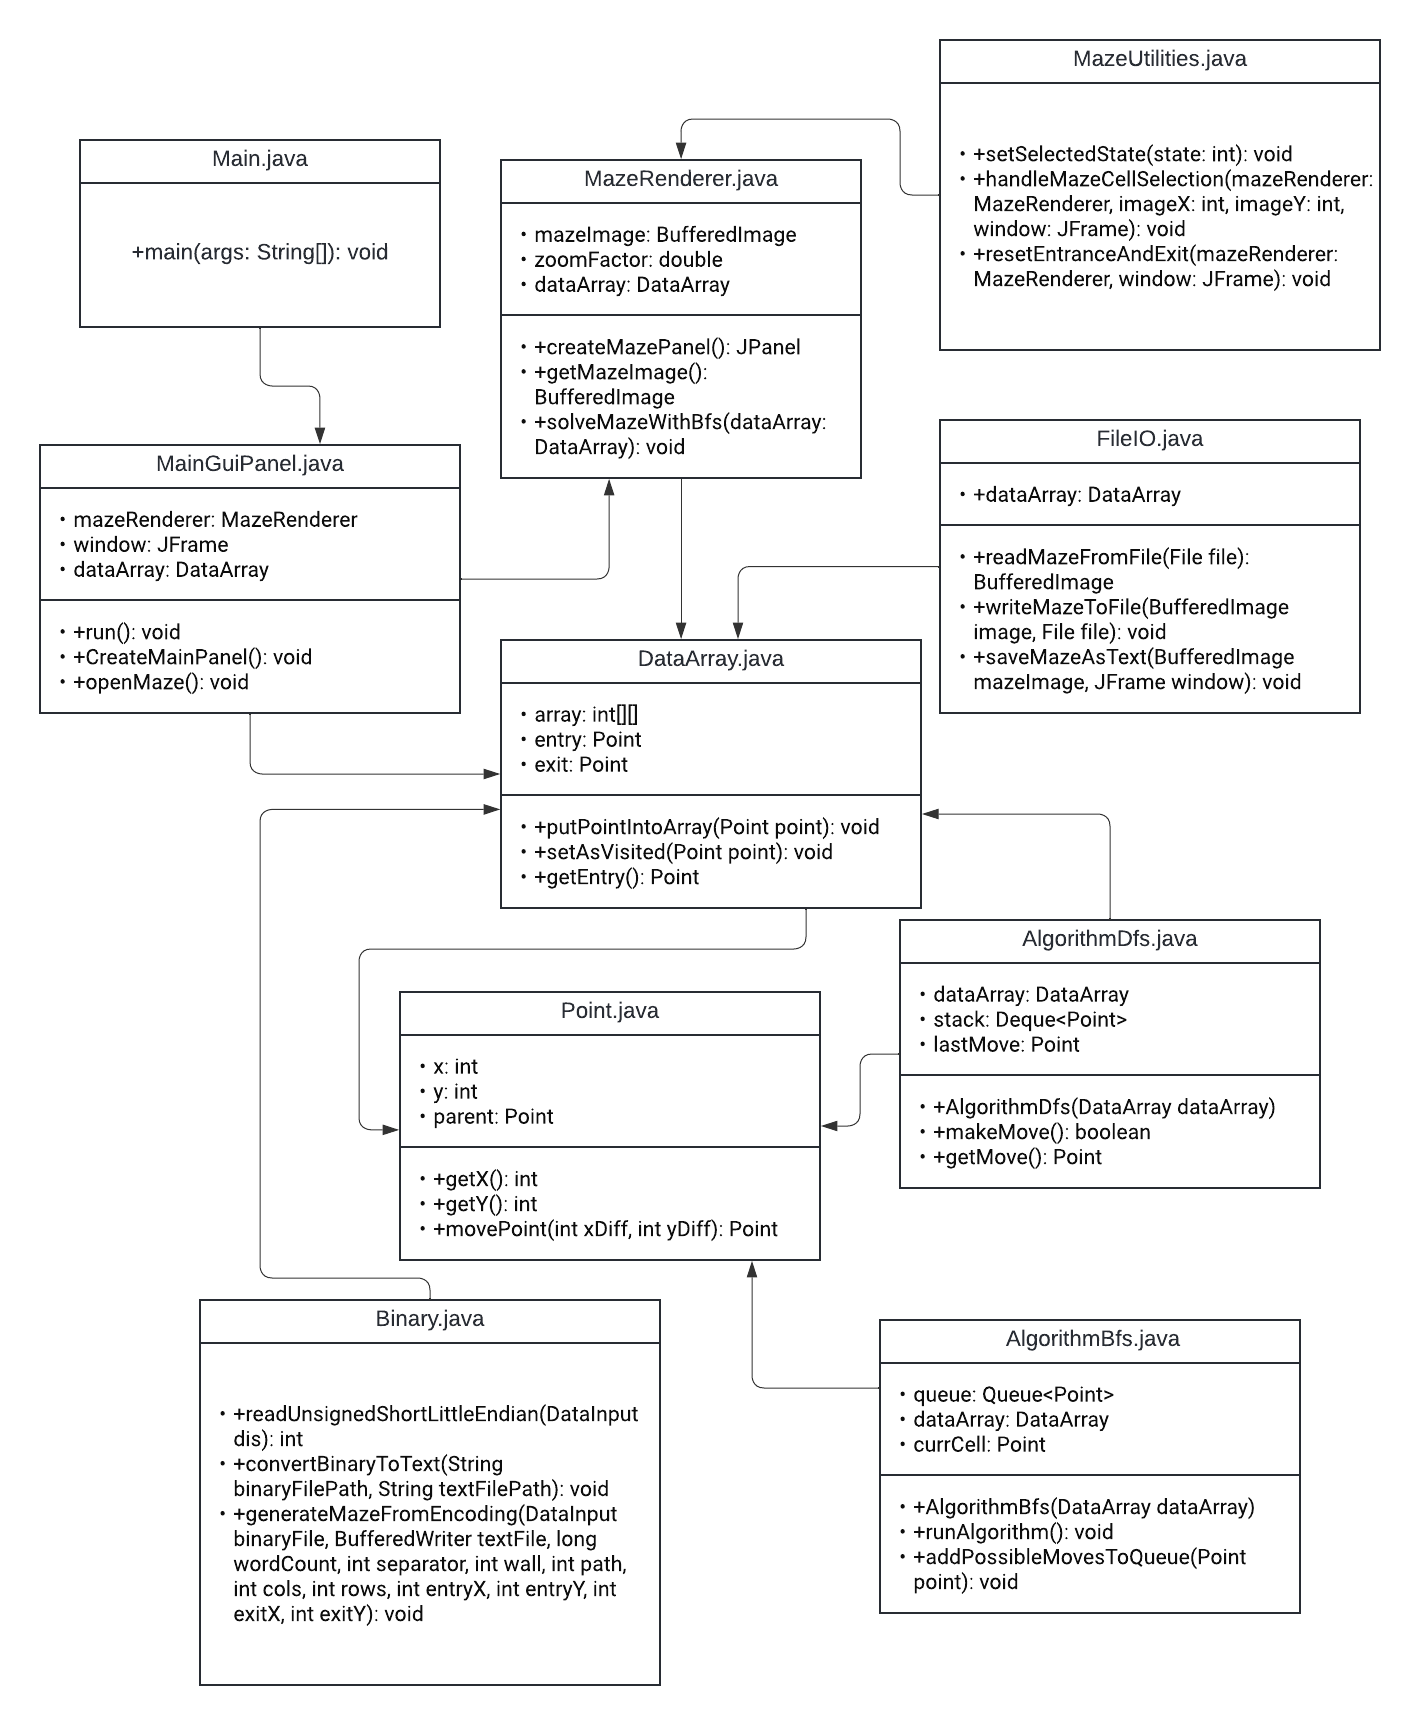
\includegraphics[width=\textwidth]{UML class.png}
    \begin{center}
        \caption{Rys.1 Diagram Klas projektu}
    \end{center}
\restoregeometry

\section{Instrukcja użytkownika}

Instrukcja użytkownika opisuje kroki, jakie należy wykonać, aby skorzystać z programu do rozwiązywania labiryntów w języku Java. Program ten pozwala na wczytanie labiryntu z pliku, wybranie algorytmu rozwiązania (BFS lub DFS), a następnie uruchomienie algorytmu w celu znalezienia ścieżki od wejścia do wyjścia. Poniżej przedstawiono szczegółowe instrukcje dotyczące korzystania z aplikacji.

\subsection{Wymagania środowiskowe}
Aby uruchomić program, należy mieć zainstalowane:
\begin{itemize}
    \item Java Development Kit (JDK) w wersji 11 lub nowszej,
    \item System operacyjny: Windows, macOS lub Linux.
\end{itemize}

\subsection{Instalacja}
\begin{enumerate}
    \item Pobierz pliki projektu z repozytorium lub innego źródła.
    \item Rozpakuj pobrane archiwum do wybranego katalogu.
    \item Otwórz terminal lub wiersz poleceń i przejdź do katalogu z projektem.
\end{enumerate}

\subsection{Uruchomienie programu}
\begin{enumerate}
    \item Skonfiguruj środowisko uruchomieniowe:
       \begin{itemize}
           \item Upewnij się, że zmienne środowiskowe JAVA\_HOME oraz PATH są poprawnie ustawione.
       \end{itemize}
    \item Otwórz katalog zawierający plik Main.java:
    \begin{verbatim}
    cd src\main\java
    \end{verbatim}
    \item Skompiluj kod programu, wpisując w terminalu:
    \begin{verbatim}
    javac Main.java
    \end{verbatim}
    \item Uruchom aplikację, wpisując w terminalu:
    \begin{verbatim}
    java Main
    \end{verbatim}
\end{enumerate}

\subsection{Korzystanie z aplikacji}
\begin{enumerate}
    \item Po uruchomieniu programu, pojawi się główne okno aplikacji z menu oraz panelem do wyświetlania labiryntu.
    \item Wybierz opcję \textbf{Plik -> Otwórz labirynt}, aby wczytać labirynt z pliku tekstowego lub binarnego.
    \item Po wczytaniu labiryntu, możesz dostosować jego widok za pomocą przycisków do powiększania i pomniejszania.
    \item Ustaw punkty wejścia i wyjścia, klikając na odpowiednie komórki labiryntu:
        \begin{itemize}
            \item Wybierz opcję \textbf{Opcje -> Ustaw wejście i wyjście}.
            \item Kliknij na wybraną komórkę na krawędzi labiryntu, aby ustawić punkt wejścia (oznaczony jako P).
            \item Następnie kliknij na inną komórkę na krawędzi labiryntu, aby ustawić punkt wyjścia (oznaczony jako K).
        \end{itemize}
    \item Wybierz algorytm, którym chcesz rozwiązać labirynt:
        \begin{itemize}
            \item \textbf{Opcje -> Znajdź najkrótszą ścieżkę (BFS)}, aby użyć algorytmu przeszukiwania wszerz.
            \item \textbf{Opcje -> Wizualizuj szukanie ścieżki (DFS)}, aby użyć algorytmu przeszukiwania w głąb.
        \end{itemize}
    \item Po znalezieniu ścieżki, wynik zostanie wyświetlony na panelu z labiryntem.
    \item Możesz zapisać wynikowy labirynt do pliku, wybierając odpowiednią opcję z menu \textbf{Plik}:
        \begin{itemize}
            \item \textbf{Zapisz labirynt (txt)}, aby zapisać labirynt w formacie tekstowym.
            \item \textbf{Zapisz obraz labiryntu}, aby zapisać labirynt jako obraz (PNG, JPEG, BMP).
        \end{itemize}
\end{enumerate}

\subsection{Resetowanie i zatrzymywanie wizualizacji}
\begin{itemize}
    \item Aby zresetować ustawione ścieżki, wybierz \textbf{Opcje -> Resetuj ścieżki}.
    \item Aby przerwać trwającą wizualizację, również wybierz \textbf{Opcje -> Resetuj ścieżki}.
\end{itemize}

\subsection{Zamykanie programu}
Aby zamknąć program, kliknij przycisk zamknięcia okna.


\section{Podsumowanie}

Projekt, którego celem było opracowanie programu w języku Java, zdolnego do znajdowania ścieżek w labiryntach, został zrealizowany z sukcesem. Dzięki zastosowaniu algorytmów DFS oraz BFS, program jest w stanie skutecznie nawigować przez labirynty o różnych rozmiarach i złożonościach. Modularna architektura systemu oraz efektywne zarządzanie pamięcią pozwoliły na osiągnięcie wysokiej wydajności oraz skalowalności rozwiązania.

\vspace{5mm}

Podczas pracy nad projektem zdobyliśmy cenne doświadczenie w zakresie implementacji zaawansowanych algorytmów nawigacyjnych, zarządzania pamięcią w języku Java oraz testowania oprogramowania. Projekt ten stanowi solidną podstawę dla dalszych prac nad bardziej zaawansowanymi systemami nawigacyjnymi i optymalizacyjnymi.

\end{document}